\documentclass[../Results.tex]{subfiles}

\begin{document}
In this section we present the maps for flux-weighted velocity and flux-weighted dispersion of Ly$\rm \alpha$, HeII and CIV emissions produced with the 3D mask to get an indication of kinematic patterns. We note that Ly$\rm \alpha$ resonant scattering effect doesn't play an important role on kinematics seen in the central area because it tends to disrupt the coherency of kinematics instead of enhancing it \citep{Cantalupo2005Fluorescent}, this is also confirmed by the results of HeII and CIV emissions.

Fig. \ref{kinematicsmap} shows the two moment maps together with the optimally-extracted images of the three emissions. The optimally-extracted images in left panel clearly shows the projected physical scale of Ly$\rm \alpha$ emission extends to 175 kpc which approximates the typical size of dark matter halo at this redshift. This projected scale is smaller comparing to the results of \citet{cai2017discovery} due to small FoV ($\rm 20\arcsec \times 33\arcsec$) of KCWI. In addition, HeII and CIV emission also extends to tens of kiloparcsec surpassing the typical size of galaxies, especially CIV emission which extends to 88 kpc. This spatially widely extended metal emissions are rarely seen at high redshift with such large projected scale.

In the middle and right panel we present the maps of first and second moment of flux distribution. The middle panel represents the flux-weighted centroid velocity maps, it shows that the velocity gradients are evident in the three maps with same direction from the northwest to the southeast. This kinematic pattern is usually the indication of rotating gas disk in CGM or outflow ejected from central AGN. Besides, the velocity map of Ly$\rm \alpha$ emission also shows gradient around G-5 from northeast to southwest.  The velocity dispersion map of Ly$\rm \alpha$ emission shows that the area around source-B possesses larger velocity dispersion ($\rm \sigma_{v} > 400 \ km/s$) and extends to $\rm 100 \ kpc$, dispersion even larger than 650 km/s which corresponds to FWHM of 1550 km/s in some spatial positions. Following the same method in \citet{Arrigoni_Battaia_2018} the expected velocity dispersion calculated for a dark matter halo hosting quasars is 300 km/s with the results $\rm M_{DM} \approx 10^{15.2} \ M_{\odot}$ in \citet{arrigoni2018overdensity} where $M_{DM}$ is the mass of dark matter halo. The significant comparison between expected dispersion and our results may indicate that there is extremely powerful kinematic activity in this region which is impossibly caused by rotation or inflow.

Fig. \ref{slices} shows the channel map of Ly$\rm \alpha$ emission with step of 200 km/s. It is clearly seen that the red component and blue component are on either side of source-B. Besides, We also extract the spectra which are normalized and fitted with one-component gaussian function of different spatial positions from circular aperture with radius of $\rm 1.5 \arcsec$ and show it in Fig. \ref{spectralss}. No significant symmetric doublets existing in the spectra confirms that the resonant scattering effect is negligible. 

Based on the above analysis, we rule out the possibility that the kinematic pattern is result from rotating gas disk, inflow and resonant scattering effect of Ly$\rm \alpha$ emission. Together with the existing of extended HeII CIV and OIII emission \citep{cai2017discovery}, the most natural and straightforward interpretation is that there is extremely powerful and widely influenced outflow ejected from source-B which has the ability to influence the entire gas environment in dark matter halo hosting source-B. The large-scale feedback effect has been widely reported before, however these observations mainly focus on the central galaxies of low redshift clusters and they are mostly powered by jet with significant radio signal. So, the halo-scale-influenced outflow with no strong radio signal at high redshift makes our observation extremely unique. So understanding the mechanism powering this strong outflow in our observation is essential for feedback effect on galaxy evolution.  

	 \begin{figure*}[htp]
		\centering
		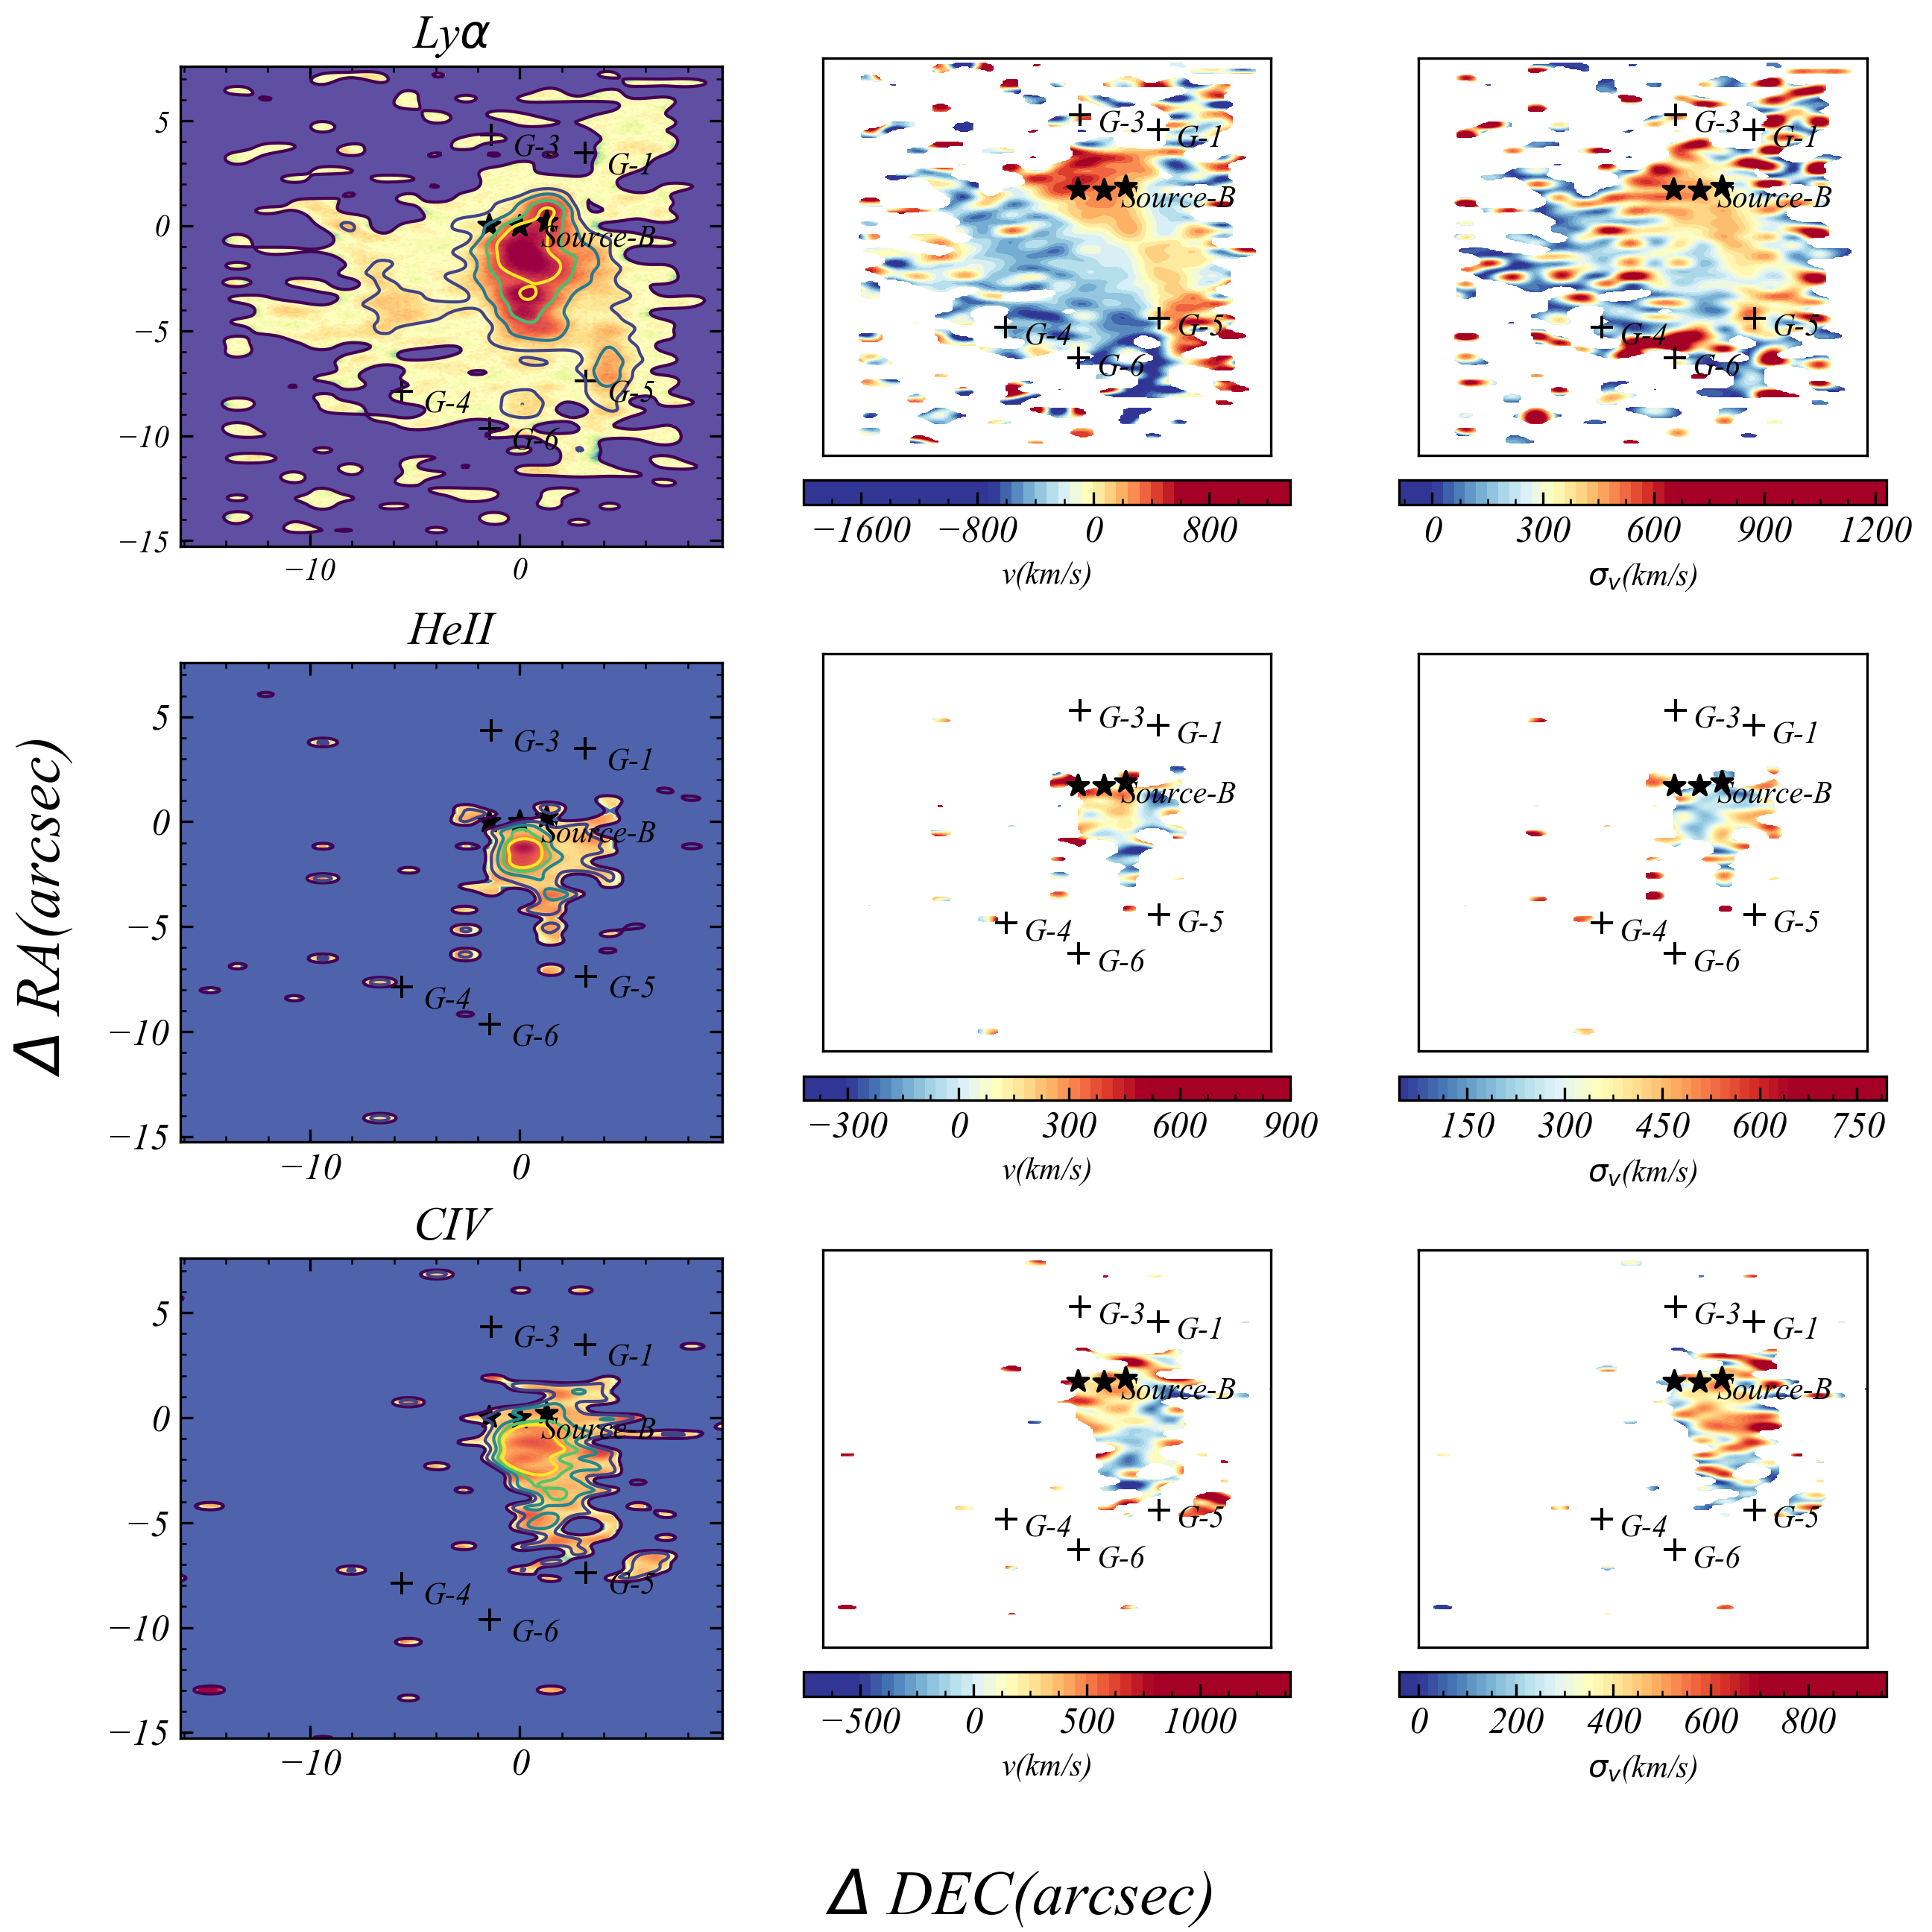
\includegraphics[width=\textwidth]{figs/emissionmap}
		\label{kinematicsmap}
		\caption{Left: continuum-subtracted psudo-narrow band images for the 3 emissions. We select regions $> 1.5\sigma$ in each slice and stack these slices together. The contour represent signal-to-noise ratio(SNR), for ly$\alpha$ is ($5\sigma,9\sigma,18\sigma,30\sigma,42\sigma,51\sigma$), for HeII is ($3\sigma,5,9\sigma$) and for CIV is ($4\sigma,7\sigma,9\sigma$). Middle: flux-weighted velocity map with respect to the systemic redshift of MAMMOTH-1. Right: flux-weighted velocity dispersion also with respect to systemic redshift of MAMMOTH-1. We also mark sources in the field with cross.}
	\end{figure*}
	
	\begin{figure*}[htp]
		\centering
		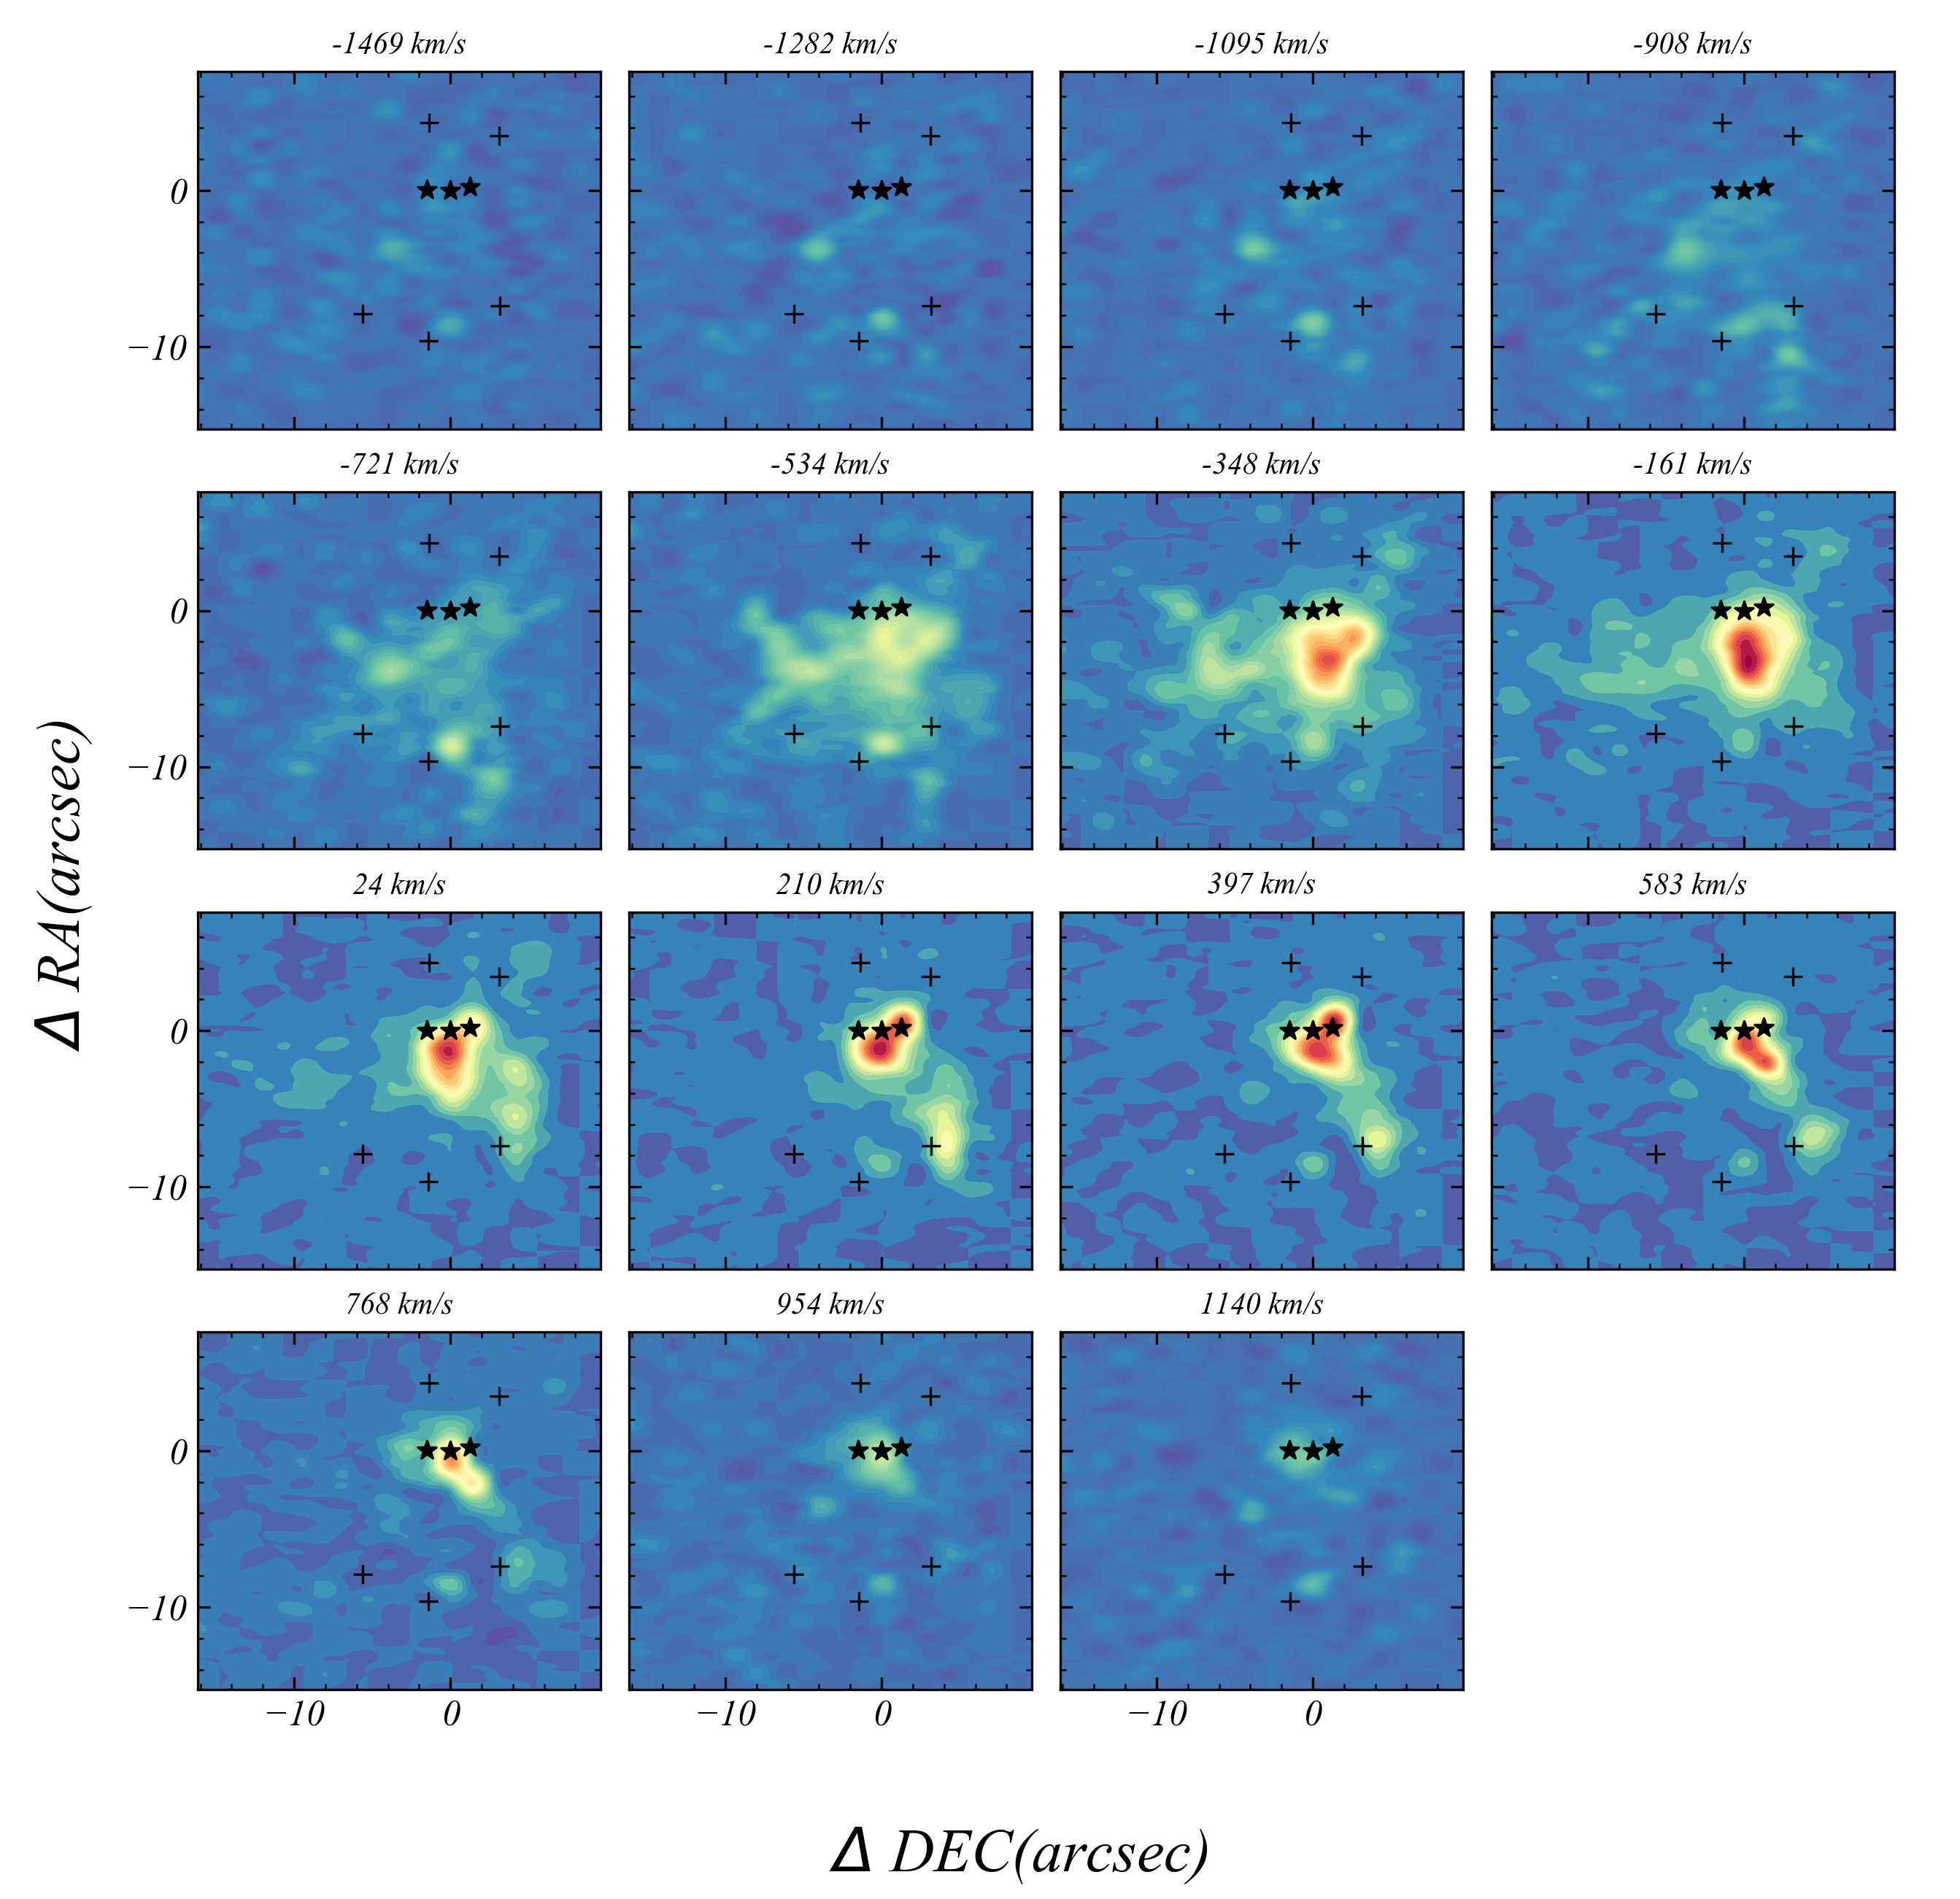
\includegraphics[width=\textwidth]{figs/slices}
		\label{slices}
		\caption{Kinematics of cool gas. It shows signal of ly$\alpha$ emission at different velocities. We select $\Delta v=187$km/s which corresponds 4$A$  as the bin size of these slices. We extract these slices within the range $4000A-4040A$, for each image here, we use the mean velocity of the bin as title for each image. It shows significant red and blue component on either side of source-B.}
	\end{figure*}
	
	\begin{figure*}[htp]
		\centering
		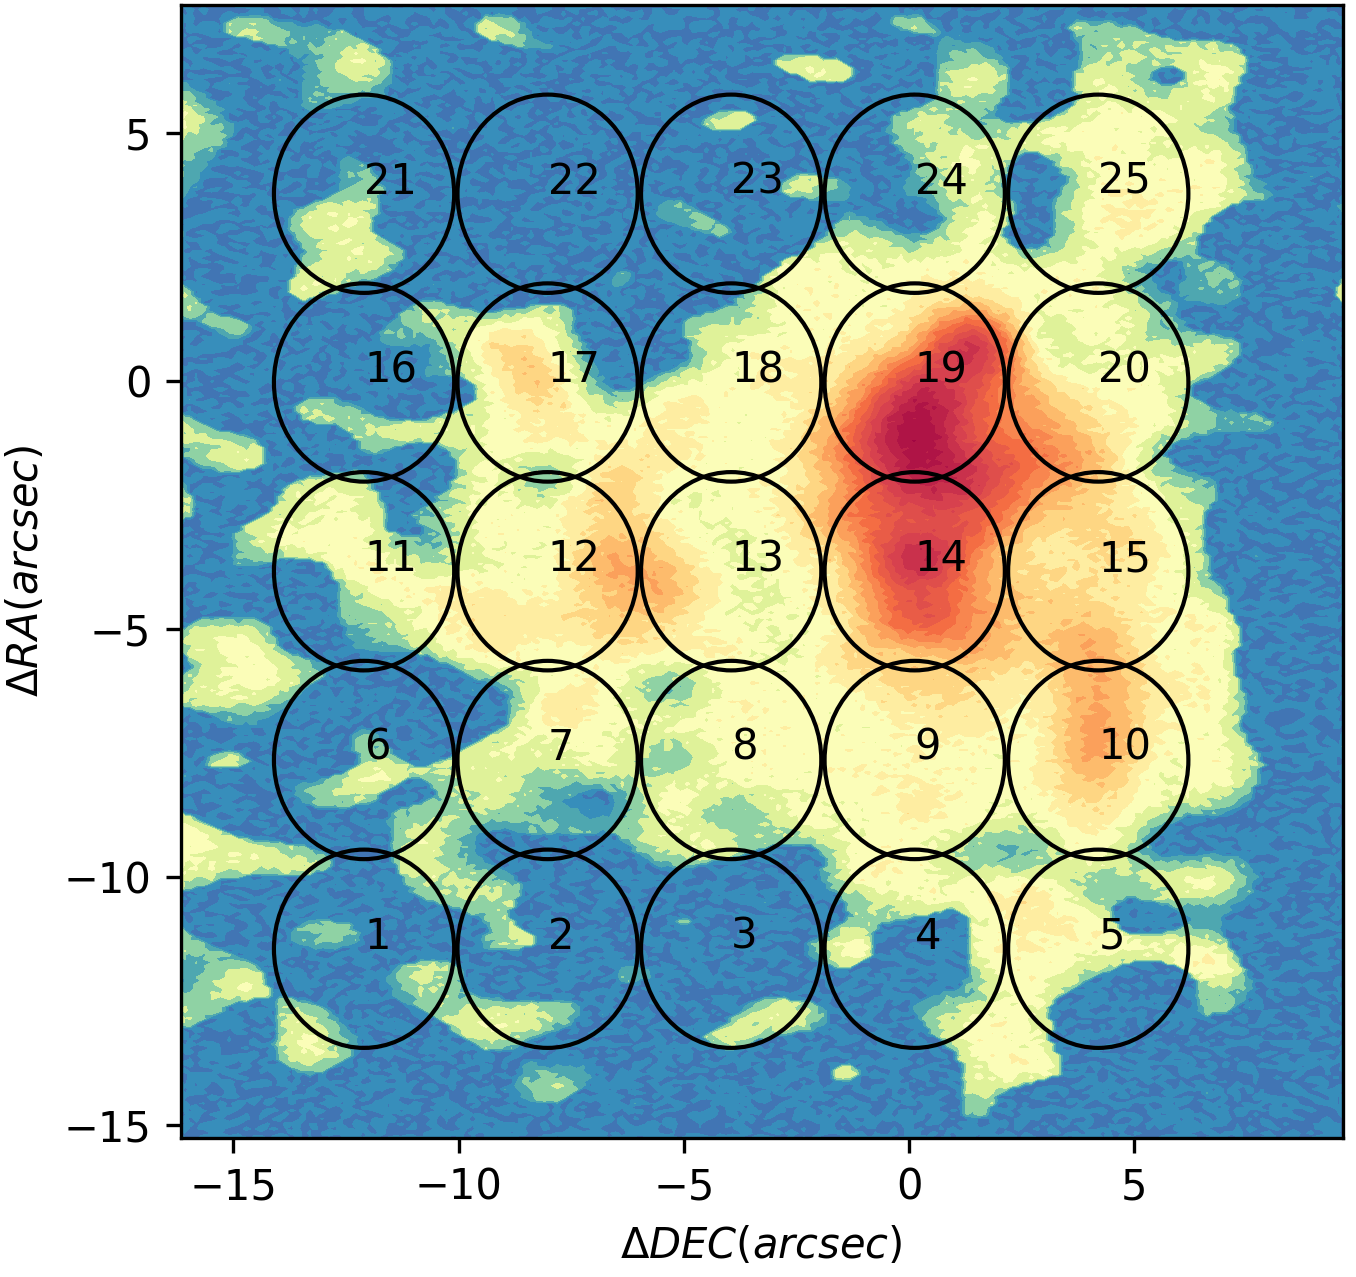
\includegraphics[width=0.5\textwidth]{figs/apertmap.png}
	\end{figure*}
	\begin{figure*}[htp]
		\centering
		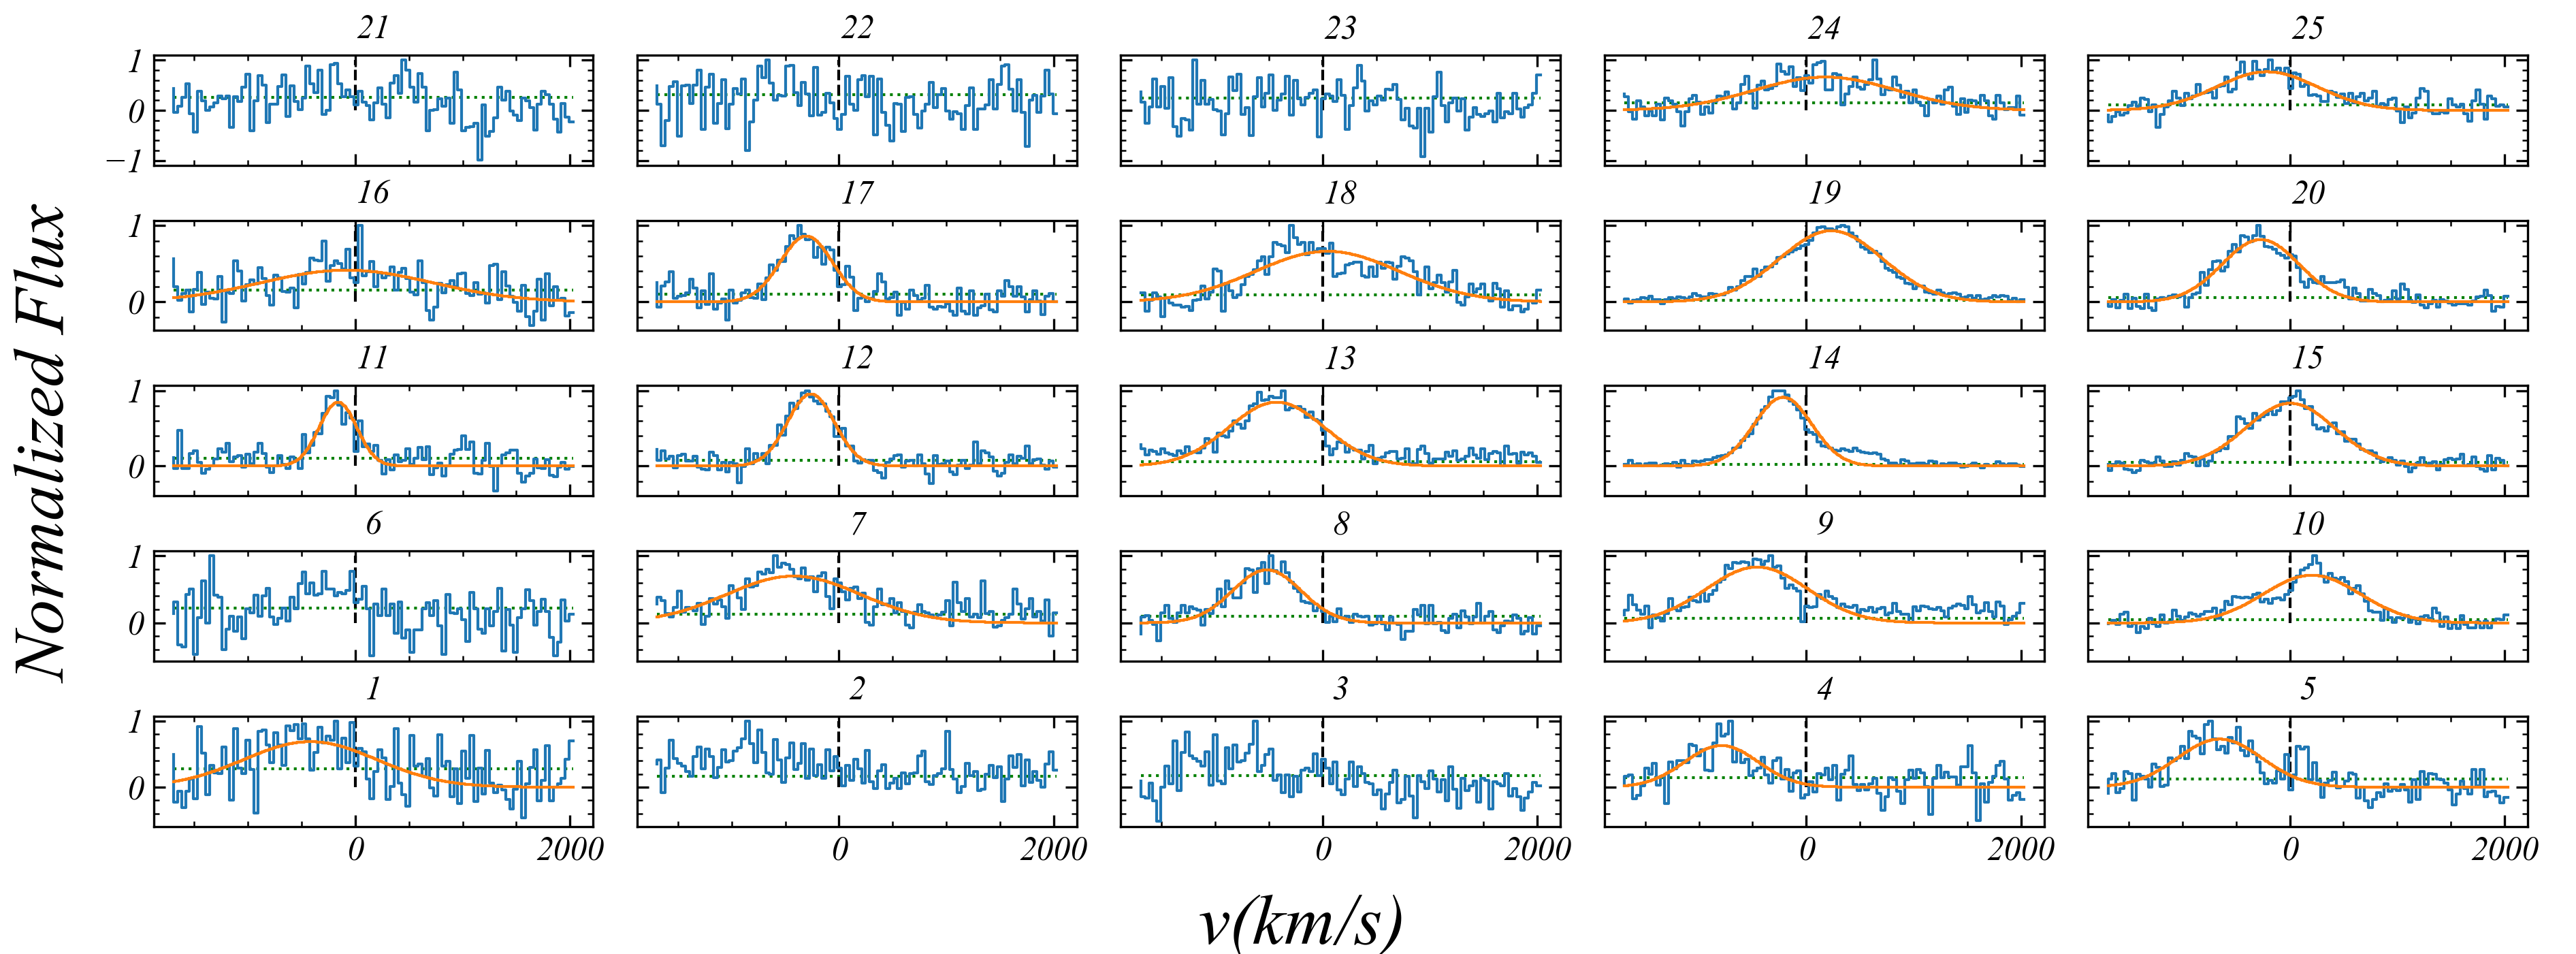
\includegraphics[width=\textwidth,height=0.45\textwidth]{figs/specmap}
		\label{spectralss}
		\caption{Up: Continuum-subtracted psudo narrow band image of ly$\alpha$. We overlay circles on it and number them from 1 to 25.  Low: Continuum-subtracted spectra extracted from individual spatial regions indicated in upper panel. The apertures are circle with radius of 2$arcsec^{2}$. We number the spectra from 1 to 25 which corresponds to circles in upper panel. We fit the emission line with single gaussian function and show it with orange lines. The green lines show the noise level calculated from the high-frequency component of spectra. }
	\end{figure*}
\begin{center}
\begin{table*}[htp]
\begin{tabular}{llllllllllllllllllll}
\hline
\hline
Number & 1    & 4    & 5    & 7    & 8    & 9    & 10   & 11   & 12   & 13   & 14   & 15  & 16   & 17   & 18   & 19   & 20   & 24   & 25   \\
\hline
Velocity(km/s)   & -416 & -785 & -649 & -419 & -515 & -453 & 208  & -157 & -257 & -424 & -211 & 9    & -75  & -300 & 49   & 236  & -267 & 182  & -208 \\
Dispersion(km/s) & 618  & 342  & 392  & 626  & 319  & 474  & 450  & 174  & 219  & 444  & 269  & 415  & 799  & 242  & 668  & 481  & 358  & 660  & 472  \\
$f_{norm}$       & 0.69 & 0.63 & 0.73 & 0.70 & 0.79 & 0.83 & 0.71 & 0.84 & 0.95 & 0.85 & 0.91 & 0.83 & 0.41 & 0.86 & 0.66 & 0.93 & 0.81 & 0.66 & 0.77 \\
\hline
\end{tabular}
\label{fitpara}
\end{table*}
\end{center}
	
\end{document}